%\documentclass{recpad2k}
\documentclass[extendedabs]{recpad2k}

\usepackage{enumitem}
\usepackage{graphicx}
\usepackage[utf8]{inputenc}

\title{Assignment 2: The Raven Test \\ \LARGE{In Search for Group Differences}}

% Enter the paper's authors in order
% \addauthor{Name}{email/homepage}{INSTITUTION_CODE}
\addauthor{Filipe Pires}{85122}{1}
\addauthor{João Alegria}{85048}{1}
\addauthor{Ana Tomé}{ana@ua.pt}{12}

% Enter the institutions
% \addinstitution{Name\\Address}
\addinstitution{
   Department of Electronics, Telecommunications and Informatics,\\
   University of Aveiro, Portugal
}
\addinstitution{
   Institute of Electronics and Informatics Engineering of Aveiro,\\
   University of Aveiro, Portugal
}

% Any macro definitions you would like to include
% These are not defined in the style file, because they don't begin
% with \bmva, so they might conflict with the user's own macros.
% The \bmvaOneDot macro adds a full stop unless there is one in the
% text already.
\def\eg{\emph{e.g}\bmvaOneDot} 
\def\Eg{\emph{E.g}\bmvaOneDot}
\def\etal{\emph{et al}\bmvaOneDot}

%------------------------------------------------------------------------- 
% Document starts here
\begin{document}

\maketitle

\begin{abstract} %%%%%%%%%%%%%%%%%%%%%%%%%%%%%%%%%%%%%%%%%%%%%%%%%%%%%%%%%%%%%%%%%%%%%%%%%%%%%%%%%%%%%%%%%%%%%%%%%%%%%%%%%%%%%%%%%%%%%%%%%%%%%%%%%%%%%%%%%%%%%%%
   \vspace{-10pt}
   {\bf 
      The search for trustworthy methodologies of determining a measurable intelligence index has been a quest of our brightest minds for decades.
      Raven matrices tests have proved to have widespread practical use as a measure of intelligence.
      They are a source of data for many studies on the general population as they seem promising tools for contexts such as psychometric tests or clinical assessment.

      In one study on the application of these matrices to groups of students from different backgrounds, questions emerged regarding the possibility of clear 
      differences between Multimedia and Informatics students.
      In this paper we present the statistical analysis applied to the tests results with the help of ML classification techniques in search for determining 
      whether any of the two groups showed significant advantages over the other.
   }
\end{abstract} 

%------------------------------------------------------------------------- 

\section{Introduction} %%%%%%%%%%%%%%%%%%%%%%%%%%%%%%%%%%%%%%%%%%%%%%%%%%%%%%%%%%%%%%%%%%%%%%%%%%%%%%%%%%%%%%%%%%%%%%%%%%%%%%%%%%%%%%%%%%%%%%%%%%%%%%%%%%%%%%%%%

Raven's Advanced Progressive Matrices (RAPM) is a non-verbal group test typically present in educational or clinical settings, as it is used in measuring 
abstract reasoning and regarded as an estimate of fluid intelligence \cite{rapm}.
Examples of related tests are Naglieri Nonverbal Ability or Spacial Ability Tests.
Their practical use is very extended, and applicable to both adults and children.
Nevertheless, studies that resort to them usually focus on populations containing groups with specific differences in order to draw conclusions from these differences.
Examples of these studies are on different military sections, or different mental disabilities.

In the study whose collected data was used for our analysis \cite{study}, the aim was to compare students from different fields in terms of learning styles effectiveness.
Several tests such as Kolb and VAK or Hermann dominances allow to distinguish some learning styles like: Accommodator, Assimilator, Auditory, Convergent,
Divergent, Kinesthetic and Visual.
But beyond this, the researchers also applied the RAPM tests to reach more robust conclusions, and combine all results in a meaningful way.
In this paper we focus only on the data related to the second set of tests.

The population that performed the Raven tests was a group of 45 university students, 21 of Design and Multimedia and 24 of Informatics Engineering.
48 problems were presented to both populations, divided into 2 phases: during the first 12, the participant would receive a feedback about his/her answer; 
for the remaining 36 no feedback was given.
During test execution, electroencephalographic (EEG) signals were registered while participants performed the tasks, using Enobio 8 EEG recording headset and 8 
channels: \textit{F3, F4, T7, C3, Cz, C4, T8} and \textit{Pz}.

Our aim was to determine from this estimated measurement of intelligence whether both groups hold characteristics significantly different from each other by 
building classification algorithms that interpret the EEG signals and other time-related metrics as features and attempt to predict which class of students a 
new entry belongs to.
We also intended to compare our conclusions with those obtained by the original researchers.

\section{Dataset \& Feature Extraction} %%%%%%%%%%%%%%%%%%%%%%%%%%%%%%%%%%%%%%%%%%%%%%%%%%%%%%%%%%%%%%%%%%%%%%%%%%%%%%%%%%%%%%%%%%%%%%%%%%%%%%%%%%%%%%%%%%%%%%%%

The dataset provided for this assignment had data both related to individual participants and aggregations with averages.
For our intentions, we were interested only in the individual results, so we used the data from the "Trial" folder, containing 4 XML spreadsheets: two for the 
Informatics students (referred to as DEI), two for the Multimedia students (referred to as ESEC).
Departments were split as one file contains the right answers of the students on the Raven tests and the other contains the wrong answers.

Each file contains information about 36 task executions, with an entry for each student and a column for each metric. 
The relevant marks for the signal analysis are around: 
\begin{itemize}[noitemsep,nolistsep]
\item Problem Display
\item Possible Solutions Display
\item Student's Answer
\end{itemize}
\vspace{2pt}
On the problem and possible solutions displays, the considered signal processing window was [-75 500] ms.
On the student's answer, the window was [-500 500] ms.

Some of the considered metrics were:
\begin{itemize}[noitemsep,nolistsep]
\item Peak \& Latency for P100 PZ, P100 CZ, P300 CZ signals
\item F3, F4 Stress signals
\end{itemize}
\vspace{2pt}
P100 and P300 were chosen because of attentional and relationship characteristics that have sometimes been attributed to them.
They are defined in the first time interval and their latency and amplitudes are stored, considering only the relevant channels.
This data was used as time features for the classification algorithms.

For the frequency features, the energy of the characteristic bands is estimated in all defined windows.
This Engergy (E) is then used to compute other higher level features called energy ratios, considering several signal channels:
\begin{itemize}[noitemsep,nolistsep]
\item Stress Index
\item Mental Fatigue
\item Alpha Lateralization
\item Immersion Index
\end{itemize}
\vspace{2pt}
All of these features are present in the dataset spreadsheets.

As in any classification challenge, we needed to divide the data into training and testing entries.
The way we divided the results was 80\% for the training of the classifiers and 20\% for testing, due to the relatively reduced size of the dataset.

\section{Data Quality \& Normalization}\label{data} %%%%%%%%%%%%%%%%%%%%%%%%%%%%%%%%%%%%%%%%%%%%%%%%%%%%%%%%%%%%%%%%%%%%%%%%%%%%%%%%%%%%%%%%%%%%%%%%%%%%%%%%%%%%

The first thing we did with the raw data was to correlate every possible pair of features through 2-Dimensional projections.
This would help us understand how was the data distributed in the multidimensional space and whether there were clear separations between the two classes 
(DEI and ESEC).
Table \ref{fig:feature} is the visual representation of this correlation as an organized collection of:
\begin{itemize}[noitemsep,nolistsep]
\item Histograms - presented in the diagonal composed by the feature related with itself and describing the value distribution inside that given feature.
\item Scatter Plots - presented in all other entries and describing the value distribution between feature pairs.
\end{itemize}

Through the analysis of this table, we can gather some important conclusions. 
The most clear characteristic detected was the presence of outliers, one that was already expected and needed to be taken care of.
The second was the fact that in all pairs of features the data doesn't appear to be separable, i.e. there should be something resembling two groups or point clouds,
one for each class, in some of the projections.
If this was visible, the possibility of actually existing a difference between groups would be likelier to be true.
However, that does not seem to be the case, since in most cases we are presented with uniform distributions, gaussian distributions or simply the grouping of 
all data in a unique central point. 
It is important to mention that this does not automatically mean that a solution could not be found, as the group distinction we were looking for could depend 
on more than two variables and so could indeed not be visible in the 2-Dimensional projections.

Once familiarized with the data, we proceeded to pre-processing it so that the models we intended to to apply would have the best chances of finding the 
distinguishing factors.
To do this, we centered the data and removed the detected outliers.
Equation \ref{zscore} contains the formula of the \textit{Z-Score} algorithm applied to each feature to center all values.
Then, we removed any data entry that contained a \textit{Null} value, since that would cause problems for the models' processing.
Finally we removed the still existing outliers with the help of equation \ref{outliers}, that ensures that entries with very distant values from the standard 
deviation are not considered as they do not have valuable information to offer.

\vspace{-5pt}
\begin{equation}\label{zscore}
   z_{i} = \frac{x_{i} - \mu}{\delta}
\end{equation}
\vspace{-10pt}
\begin{equation}\label{outliers}
   |x_{i}-\mu| < 3\times\delta
\end{equation}
\vspace{-10pt}

\section{Classifiers}\label{classifiers} %%%%%%%%%%%%%%%%%%%%%%%%%%%%%%%%%%%%%%%%%%%%%%%%%%%%%%%%%%%%%%%%%%%%%%%%%%%%%%%%%%%%%%%%%%%%%%%%%%%%%%%%%%%%%%%%%%%%%%%

In this section we will present a brief summary of all the machine learning (ML) models used in this study. 
We chose these models since, through a state-of-the-art analysis, we concluded that these are the most common and suggested models and the ones that 
usually achieve the best performance overall in ML problems. 
We also found some of the models used are the most recommended when handling data similar to our context.

The implementation of the mentioned ML models was done in Python, using Jupyter Notebooks in order to organize and share both the analysis descriptions, 
the code and the results.
In the git repository \footnote{\url{https://github.com/joao-alegria/EDRaven}}, the reader can find the developed notebooks and their execution requirements.

\subsection{Support Vector Machine} 

\textit{Support Vector Machine}, commonly denoted as SVM, is a supervised ML model that maps the different data entries into a multidimensional 
space with the supplied training set in a way that the widest possible gap exists between the data of each class. 
Based on that gap, a model is created and a decision rule defined so that, when fed with new data, it tries to assign a class to it by comparing the information 
against the defined decision rule.

The most common and simple SVM application tries to creates a linear division between the presented classes. Another alternative that allows more complex 
decision rules is the application of a kernel trick, that implicitly maps the data to a higher-dimensioned feature space, which may enable a better separation 
of the data.

\subsection{MultiLayer Perceptron}

\textit{MultiLayer Perceptron} (or MLP) is a class of feedforward artificial neural network (ANN), another supervised ML model. 
The basic idea behind this model is the composition of a network of multiple layers of perceptrons.
A perceptron is also a supervised learning algorithm, capable of performing binary classifications according to a linear predictor function. 
The power of MLP lies in the junction of several of these perceptrons to achieve outstanding classification performances.

This junction normally follows a standard architecture divided in layers: 
an input layer, where the features are received;
then, the data is passed to one or more hidden layers;
and finally sent to an output layer, where the classification is consolidated. 
The input and output layers are the ones that interact with the exterior.
The hidden layers are responsible for the learning process; it is mostly here where the fine-tunning of the model is applied. 
In this architecture, the number of layers andof neurons (singular cells inside a layer) can be adapted to improve the model performance.

\subsection{Decision Tree} 

This supervised learning algorithm, as the name suggests, uses a tree-like structure to support the data classification decision-making and aims to convert the 
observed patterns in the train data into conclusions about the data classes. 
The construction of this structure is straightforward, consisting in assigning a condition to each new branch so that data converges to class-separating branches 
and uni-class leafs.
The conditions must be defined with caution since a poor decision in an intermediate branch may cause a drastic decrease in the overall performance of the model. 

Many times this process uses \textit{Entropy} as a guide, since this property indicates, in a very high level approximation, the level of 
confusion/chaos/randomness of a set of information; 
thereby if the data tested belongs to only one class, the entropy should be 0 and the system knows that that data portion doesn't need to be divided anymore.

\subsection{Random Forest}

Similarly to the last model, \textit{Random Forest} also uses tree structures to support the models' classification decisions. 
The difference is that now the model uses several instances of Decision Trees, with the purpose of dividing the problem and considering the decision of all 
trees, considering that sometimes Decision Trees don't generate the best branching configuration possible and several of them combined may solve the limitations 
of singular trees.

\subsection{K Nearest Neighbors}

The last model that we decided to test was the \textit{K Nearest Neighbors} (or KNN), which is one of the simplest learning algorithms but no less relevant 
in the field of ML. 
As a supervised learning algorithm, KNN classifies data by representing every train entry in a multidimensional space; then, when presented with new data entries, 
the model represents the new multidimensional points in space and verifies the class of the K nearest points (train entries) - the most frequent class in that K 
subset is the one that is assigned to the new data entry. 

\section{Models Fine Tuning}\label{parameters} %%%%%%%%%%%%%%%%%%%%%%%%%%%%%%%%%%%%%%%%%%%%%%%%%%%%%%%%%%%%%%%%%%%%%%%%%%%%%%%%%%%%%%%%%%%%%%%%%%%%%%%%%%%%%%%%%

\subsection{Performance Evaluation}

Once the classification models were implemented, we needed to measure their performance.
This was accomplished through the confusion matrix, a matrix that correlates a model's predictions with the true values and gives us the number of: 
true positives (TP) and true negatives (TN), the correct predictions of wether an entry belongs to 1 of the classes or not; false positives (FP) and 
false negatives (FN), the incorrect predictions.
The class defined as true can be any of the two, as the process is equivalent when inversed.
In our case this was done internally by library sklearn \cite{sklearn}.
With these values, we were able to compute 4 performance metrics:
\begin{itemize}[noitemsep,nolistsep]
\item Accuracy, given by $A = \frac{TP + TN}{TP + TN + FP + FN}$
\vspace{3pt}
\item Precision, given by $P = \frac{TP}{TP + FP}$
\vspace{3pt}
\item Recall, given by $R = \frac{TP}{TP + FN}$
\vspace{3pt}
\item F1-Score, given by $F = \frac{2 \times P \times R}{P + R}$
\vspace{3pt}
\end{itemize}
During our analysis we only consider \textit{A} and \textit{F}, as accuracy alone is not enough to evaluate the models (not robust to several aspects) and F1 
correlates precision and recall very effectively.

\subsection{Parameters Variation}

In this section we present the manipulation of the hyperparameters related to each of the implemented algorithms, in search for better performances.

For the SVM, using the default parameters with the Radial Basis Function (RBF) kernel, the accuracy was around 55\%.
The sigmoid kernel proved to be more appropriate for the dataset as it increased both the accuracy to 57\% and the F1-Score from 68\% to about 73\%.
The remaining parameters such as the kernel coefficient (altered between "auto" and "scale"), tolerance for stopping criterion (ranged from $1.0 \times 10^{-3}$
to $0.1$), decision function shape or maximum number of iterations proved to have no significant effect when carefully altered.

Moving on to MLP, the default parameters of the ANN were the following:
"relu" activation layer, "adam" solver for weight optimization, L2 penalty and tolerance both at $1.0 \times 10^{-4}$, "constant" learning rate and an 
architecture with 3 hidden layers of 13 nodes.
This configuration resulted in an accuracy of 54\%.
The best found configuration turned out to be the following: "identity" activation layer (although not very different from the original), "lbfgs" solver (that 
proved to be more effective than "adam" for our dataset), a simples architecture with 2 hidden layers of 10 and 5 nodes (that had the same effect as the previous), 
and the remaining parameters kept the default values (as changing them only reduced the performance).
The final performance was of 56\% of accuracy and 67\% of F1-Score.

The DTs showed worse results in all metrics.
Changing the criterion (function to measure the quality of a split) from "gini" to "entropy" showed no improvements, nor did tweaking the trees' maximum depth 
or minimum number of samples required to split an internal node.
Defining the weights associated with classes made precision fall 2 percentiles.
The best accuracy found was 53\% with F1 at 58\%.
The addition of Random Forests was an attempt to improve these values, as RFs use several DTs to return a combined answer theoretically better than one 
considering only one DT.
However, from our studies, Random Forests were only able to improve F1-Score, and only slightly with a maximum value of 60\%.

Finally we dedicated our attention to KNN.
Reducing the number of K nearest neighbors from 5 to 3 seemed to have a considerably good effect on its performance.
Also, defining the algorithm used for computing the nearest neighbors was futile, as all alternatives had no effect whatsoever.
Altering the distance calculation formula from euclidean to any other reduced the precision, so the best configuration gave an accuracy of 53\%, with F1 at 60\%.

\subsection{Feature Manipulation}

As an extra effort to try to extract or even create some additional meaningful information, we decided to generate new features based on the already existing ones. 
As a logical aggregation strategy, we decided to multiply \textit{Display} metrics with their corresponding \textit{Solutions} metric. 
This, by our interpretation, allows a finer definition of the metric itself.

After creating the new dataset and re-training all the models, we concluded that this attempt only produced minor improvements over the previous results, 
reaching sometimes increases of 5\% on the performance metrics. 
These improvements were not the ones we were looking for when adding new features, but were a good sign. 
The conclusion we reached was that the accomplished increase did not alter our results interpretation.

\section{Results Discussion} %%%%%%%%%%%%%%%%%%%%%%%%%%%%%%%%%%%%%%%%%%%%%%%%%%%%%%%%%%%%%%%%%%%%%%%%%%%%%%%%%%%%%%%%%%%%%%%%%%%%%%%%%%%%%%%%%%%%%%%%%%%%%%%%%%%

After executing all the parameter variation study, the feature analysis as well as some feature addition in hopes of adding some extra meaningful information 
to the already existing data, the best performance results were the ones presented in Section \ref{parameters}.
Although not the most satisfying results, since when conducting the development of a ML model the aim is to obtain a model with a defined set of hyperparameters 
that generate a good performance with good values(close to 100\%) on its performance indicators, but the results obtained in this study have a reason to be.

Referring to Section \ref{data}, one of the conclusions taken from analyzing the Figure \ref{fig:feature} was that no obvious division was observable in the 
data projections in the different feature pair plane. Although this conclusion not absolute proof that the data isn't separable, the results of the tested 
model indicate that that is the case. This can be caused by several reasons, ranging from the dataset quality, the models used, the tunning of the 
hyperparameters or even the case of overfitting of the training data. 

Through a deeper analysis over the data itself we didn't found any aspect that could compromise our study; the origin of the data and the metrics gathered 
seemed to be the most adequate for this type of study; the features also seemed to be widespread enough to encapsule all the possible signals related to this 
study, such as fatigue, immersion, stress, etc. In relation to the models used, as already mentioned in Section \ref{classifiers} are state-of-the-art, 
therefor should perform well enough with the dataset presented, and for that matter, with any dataset. The parameters variation was probably the portion of 
the report study that took the longer, since we made a meticulous study of the parameters for all the models trained as detailed in Section \ref{parameters}. 
For that reason we can conclude that the parameter choice is also not the problem. Finally, in relation to the overfitting problem, the fact that all the models 
used gave similar results, it's quite improbable that all of them suffer from the overfitting. That allows us to also remove this problem from our list of 
possible issues.

Knowing that the variables in our reach are properly tested and in theory are correct, we can only conclude that the data itself is inseparable. 
This means that the two classes presented, the students from \textit{DEI} and the students from \textit{ESEC}, although obviously two different groups in this 
study, the conducted experiment indicates that in terms of the \textit{RAVEN} intelligence estimation test there is no difference between the two groups.

Finally, in spite of all models produced a similar performance, where the \textit{Accuracy} averaged in the 55\% mark and the \textit{F-Score} averaged in the 
65\% mark. This difference is due to the fact that both \textit{Precision} and \textit{Recall} are slightly higher than the \textit{Accuracy}, which indicates 
that however the classification is almost random, in reality the models are able to generate more true results than negative results, which is quite interesting 
given the limitations observed from the models.

\section{Conclusions \& Future Work} %%%%%%%%%%%%%%%%%%%%%%%%%%%%%%%%%%%%%%%%%%%%%%%%%%%%%%%%%%%%%%%%%%%%%%%%%%%%%%%%%%%%%%%%%%%%%%%%%%%%%%%%%%%%%%%%%%%%%%%%%%%

Determining differences between populations is not a trivial task.
The subjectiveness element of intelligence measurements increase the complexity of such problem, and so clear conclusions are very hard to find.
Nevertheless there are many cases where, when the correct analysis tools are applied, solid conclusions are reached - even if they are precisely that 
no conclusion can be drawn - and this is exactly that case.

By discussing our results and the similarity of outcomes between very different classification models, and comparing our results with those obtained in the 
original study conducted by the dataset authors, we were able to understand that in fact there are no significant differences between Multimedia and Informatics 
students in terms of intelligence.
In fact, this is parallel to our initial suppositions, as both classes require highly cognitive skills and problem solving capacities, even though applied to 
very different situations.

For future work, we believe it would not be a good idea to attempt implementing other classification algorithms, as they would very much likely return similar results.
Instead, if the interest of analyzing the same dataset remained, we would probably address different questions such as "Are there any differences between 
women and men within these courses?", or "Is it possible to predict whether a student will get the answer right to one of the Raven's tasks or not?".

Our overall perspective on the project is very positive, even though we, as Informatics students, were wishing to find advantages on the side of the 
students with a similar background as ourselves.
Nevertheless, we found the use of Jupyter Notebooks very practical and adequate to assignments such as this and, as it allowed us to segment the work to be done,
we were able to keep a good balance and work distribution between group elements throughout the development.

%------------------------------------------------------------------------- 
% \subsection{Footnotes}

% Please use footnotes\footnote {This is what a footnote looks like.  It
% often distracts the reader from the main flow of the argument.} sparingly.
% Indeed, try to avoid footnotes altogether and include necessary peripheral
% observations in 
% the text (within parentheses, if you prefer, as in this sentence).  If you
% wish to use a footnote, place it at the bottom of the column on the page on
% which it is referenced. Use Times 8-point type, single-spaced.

%------------------------------------------------------------------------- 
% \subsection{The ruler}

% The \LaTeX\ style defines a printed ruler which should be present in the
% version submitted for review.  The ruler is provided in order that
% reviewers may comment on particular lines in the paper without
% circumlocution.  If you are preparing a document using a non-\LaTeX\
% document preparation system, please arrange for an equivalent ruler to
% appear on the final output pages.  The presence or absence of the ruler
% should not change the appearance of any other content on the page.  The
% camera ready copy should not contain a ruler. (\LaTeX\ users may remove
% the \verb'[review]' option from the \verb'\documentclass' statement.)
% Reviewers: note that the ruler measurements do not align well with lines
% in the paper --- this turns out to be very difficult to do well when the
% paper contains many figures and equations, and, when done, looks ugly.
% Just use fractional references (e.g.\ this line is $210.5$), although in
% most cases one would expect that the approximate location ($210$ in the
% previous example) will be adequate.

%------------------------------------------------------------------------- 
% \subsection{Mathematics}

% Please number all of your sections and displayed equations.  It is
% important for readers to be able to refer to any particular equation.  Just
% because you didn't refer to it in the text doesn't mean some future reader
% might not need to refer to it.  It is cumbersome to have to use
% circumlocutions like ``the equation second from the top of page 3 column
% 1''.  (Note that the ruler will not be present in the final copy, so is not
% an alternative to equation numbers).  All authors will benefit from reading
% Mermin's description~\cite{Mermin89} of how to write mathematics.

%------------------------------------------------------------------------- 

\begin{thebibliography}{00}
\bibitem{rapm} Warren B. Bilker et al., "Development of Abbreviated Nine-item Forms of the Raven’s Standard Progressive Matrices Test", \url{https://www.ncbi.nlm.nih.gov/pmc/articles/PMC4410094}, accessed in December 2019.
\bibitem{study} Felisa M. Córdova et al., "Identifying Problem Solving Strategies for Learning Styles in Engineering Students Subjected to Intelligence Test and EEG Monitoring", \url{https://www.sciencedirect.com/science/article/pii/S1877050915014787}, Procedia Computer Science 55 (2015), accessed in December 2019.
\bibitem{sklearn} Python SW Foundation, "scikit-learn 0.22", \url{https://pypi.org/project/scikit-learn/}, accessed in December 2019.
%\bibitem{assign2} A. Tomé, "Data Mining Assignment", \url{https://elearning.ua.pt/pluginfile.php/1496406/mod_resource/content/3/ED_HCT_Raven.pdf}, accessed in December 2019.

\end{thebibliography}
% https://en.wikipedia.org/wiki/Support-vector_machine
% https://en.wikipedia.org/wiki/Multilayer_perceptron
% https://en.wikipedia.org/wiki/Perceptron
% https://en.wikipedia.org/wiki/Decision_tree
% https://en.wikipedia.org/wiki/K-nearest_neighbors_algorithm

% \bibliography{recpad_review}

\appendix
\begin{figure}[h]
   \centering
   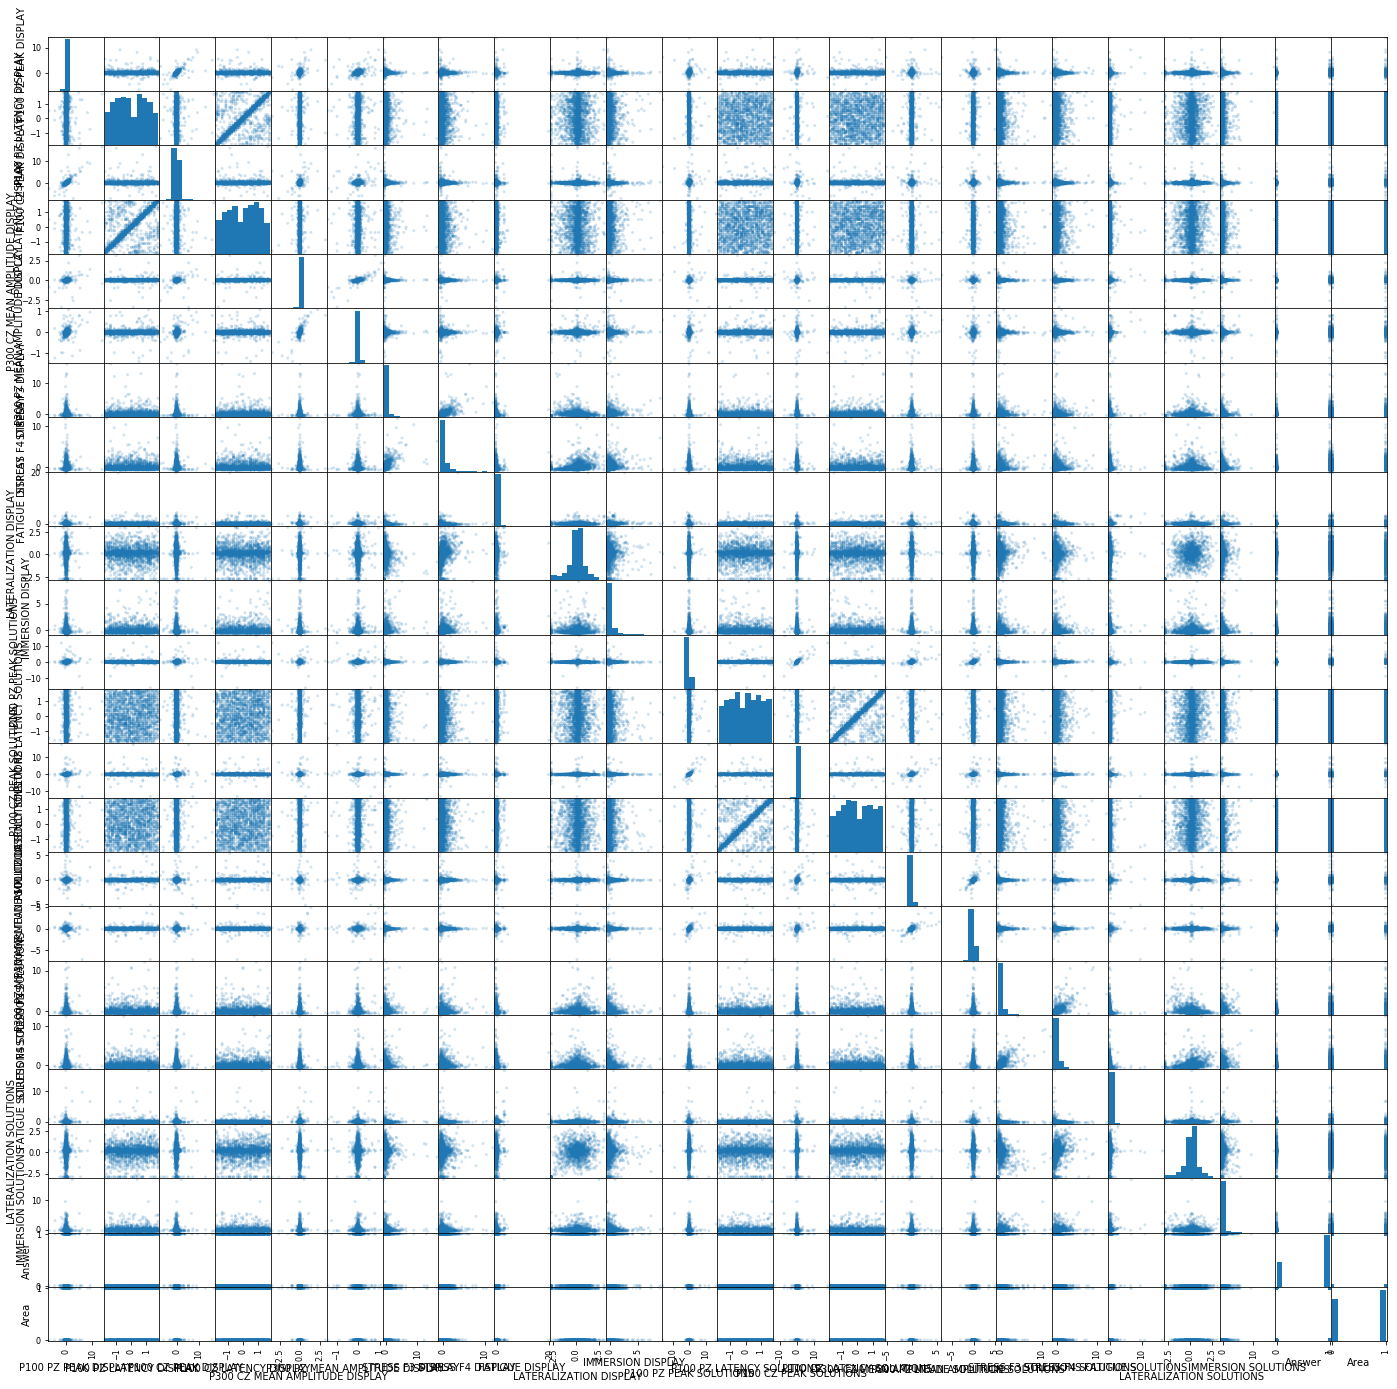
\includegraphics[width=2\linewidth]{featurecorrelation.png}
   \caption{Feature Correlations}
   \label{fig:feature}
\end{figure}

\end{document}
